\documentclass[10pt,a4paper]{article}
\usepackage[utf8]{inputenc}
\usepackage[german]{babel}
\usepackage{amsmath}
\usepackage{amsfonts}
\usepackage{amssymb}
\usepackage{siunitx}
\usepackage{multirow}
\usepackage[left=2cm,right=2cm,top=2cm,bottom=2cm]{geometry}
\usepackage{wrapfig}
\usepackage{graphicx}
\usepackage{caption}
\usepackage[colorlinks]{hyperref}


\author{Christian Bespin \and Christopher Deutsch}
\title{Übungsblatt 2: Numerische Methoden der Physik}
\begin{document}
\maketitle

\setcounter{section}{1}

\section{Skin-Effekt}

\subsection{Physikalischer Hintergrund}

In einem zylinderförmigen elektrischen Leiter mit Radius $\rho_0$, der hinreichend lang ist und in dem ein Wechselstrom $I(t)=I_0 e^{i \omega t}$ fließt, ist die Stromdichte nicht über den ganzen Leiterquerschnitt konstant. Das im Leiter schwingende elektrische Feld genügt bei verschwindendem Verschiebungsstrom ($\dot D \approx 0$) der elektromagnetischen Wellengleichung:
\begin{align}
	\Delta\mathbf{E} - \frac{4\pi\sigma\mu}{c^2} \frac{\partial \mathbf{E}}{\partial t} = 0
	\label{eq:maxwellgleichung}
\end{align}
Wir drücken das elektrische Feld $\mathbf{E}$ durch das ohm'sche Gesetz $\mathbf{j} = \sigma \mathbf{E}$ aus und separieren die Zeitabhängigkeit der Stromdichte \cite{healdmarion} indem wir $\mathbf{j} = \mathbf{j}_0 e^{i \omega t}$ setzen.
\begin{align}
	\Delta\mathbf{j}_0 + k^2 \mathbf{j}_0 = 0
	\label{eq:maxwellgleichungJ}
\end{align}
mit $k^2 = - i \frac{4 \pi \sigma \mu \omega}{c^2}$. Gehen wir in Zylinderkoordinaten über, wobei die z-Achse parallel zum Leiter gelegt wird und nutzen Symmetrie aus (keine Winkelabhängigkeit der Stromdichte), erhalten wir:
\begin{align}
	\frac{\mathrm{d}^2 j_0}{\mathrm{d}\rho^2} + \frac{1}{\rho}\frac{\mathrm{d}j_0}{\mathrm{d}\rho} + k^2 j_0 = 0
	\label{eq:besseldgl} 
\end{align}
Multiplikation dieser Gleichung mit $\rho^2$ liefert mit der Substitution $\xi = k \rho$ die Bessel'sche Differentialgleichung:
\begin{align}
  \xi^2 \frac{\mathrm{d}^2j_0}{\mathrm{d}\xi^2} + \xi \frac{\mathrm{d}j_0}{\mathrm{d}\xi} + \xi^2 j_0 = 0
\end{align}
Als allgemeine Lösung erhält man Besselfunktionen erster Art und nullter Ordnung, mit der Integrationskonstante $A$:
\begin{align}
	j_0(\rho)=A J_0(k \rho) = A(\mathrm{ber}_0(\kappa \rho)+i\mathrm{bei}_0(\kappa \rho))
\end{align}
wobei für $\kappa$, wie auf dem Blatt definiert, $\kappa = 2 \sqrt{\pi \sigma \mu \omega}/c$ gilt.
Die Konstante $A$ kann aus dem Strom, der im Leiter fließt, bestimmt werden \cite{kazimierczuk}, woraus direkt
\begin{align}
	j_0(\rho) = \frac{I_0 \kappa}{2\pi\rho_0}\frac{\mathrm{ber}_0(\kappa\rho)+i \mathrm{bei}_0(\kappa\rho)}{\mathrm{bei}'_0(\kappa\rho_0)-i\mathrm{ber}'_0(\kappa\rho_0)}
\label{eq:stromdichte}
\end{align}
folgt. Mit steigender Frequenz $\omega$ geschieht der Ladungstransport überwiegend am Rand des Leiter, weil das (alternierenden) Magnetfeld, das vom Wechselstrom induziert wird, Kraft (Lorentzkraft) auf die Ladungsträger ausübt. Diese ist zum Rand des Leiters gerichtet, weshalb am Rand mehr Ladungsträger lokalisiert sind als im Kern, wobei die Schicht am Rand des Leiters, in dem sich die Ladungsträger konzentrieren, mit zunehmender Frequenz $\omega$ immer dünner wird. Darum wird das Phänomen als \emph{Skin-Effekt} bezeichnet. Insbesondere ist $j_0$ eine komplexe Zahl, da sie nach dem Separationsansatz sowohl Amplituden- wie auch Phaseinformation enthält.

\subsection{Mathematischer Hintergrund}

\subsubsection{Bessel-Funktionen erster Art}

Man kann die Bessel-Funktionen erster Art durch ihre Potenzreihenentwicklung im Ursprung definieren:
\begin{align}
	J_\nu(z) = \sum^{\infty}_{m=0} \frac{\left( -1 \right)^m}{m! \, \Gamma(m + \nu + 1)} \left(\frac{z}{2}\right)^{2m+\nu}
\end{align}
Dabei ist $\nu \in \mathbb{R}$. Uns interessiert die Besselfunktion 0-ter Ordnung $\nu = 0$.
Mit der Identität $\Gamma(n+1) = n!$ für $n \in \mathbb{N}$ ergibt sich:
\begin{align}
	\label{eq:bessel0}
	J_0(z) = \sum^{\infty}_{m=0} \frac{\left( -1 \right)^m}{\left( m! \right)^2} \left( \frac{z}{2} \right)^{2m}
\end{align}

\subsubsection{Kelvin-Funktionen}
\label{sssec:kelvin-funktionen}

Die Kelvin-Funktionen $\mathrm{ber}_\nu(x)$ und $\mathrm{bei}_\nu(x)$ sind definiert als der Real-
beziehungsweise Imaginärteil von $J_\nu(x \sqrt{-i} )$. Mit (\ref{eq:bessel0})
folgt für den Fall $\nu = 0$ umgehend die Reihendarstellung der Kelvinfunktionen:
\begin{align}
	\mathrm{ber}_0(x) = 1 + \sum^{\infty}_{k=1} \frac{\left( -1 \right)^k}{\left( \left(2k\right)! \right)^2} \left( \frac{x}{2} \right)^{4k}&&
	\mathrm{bei}_0(x) = \sum^{\infty}_{k=0} \frac{\left( -1 \right)^k}{\left( \left(2k+1\right)! \right)^2} \left( \frac{x}{2} \right)^{4k+2}\label{eq:potenzreihe}
\end{align}
Um die erste Ableitung zu erhalten, leiten wir (\ref{eq:potenzreihe}) gliedweise ab:
\begin{align}
	\mathrm{ber}'_0(x) = \sum^{\infty}_{k=1} \frac{\left( -1 \right)^k}{\left( 2k-1 \right)! \, \left( 2k \right)!} \left( \frac{x}{2} \right)^{4k-1}&&
	\mathrm{bei}'_0(x) = \sum^{\infty}_{k=0} \frac{\left( -1 \right)^k}{\left( 2k \right)! \, \left( 2k+1 \right)!} \left( \frac{x}{2} \right)^{4k+1}\label{eq:dpotenzreihe}
\end{align}
In asymptotischer Näherung \cite{abramowitzstegun} ergibt sich mit den Definitionen $\alpha = \frac{x}{\sqrt{2}}-\frac{\pi}{8}$ und $C(x) = e^{\frac{x}{\sqrt{2}}}/\sqrt{2 \pi x} $:
\begin{align}
	\mathrm{ber}_0(x) &\approx C(x) \left[f_0(x) \cos(\alpha) + g_0(x) \sin(\alpha) \right]\label{eq:berpotenzreiheasym}-\frac{\mathrm{kei}_0(x)}{\pi}\\
	\mathrm{bei}_0(x) &\approx C(x) \left[f_0(x) \sin(\alpha) - g_0(x) \cos(\alpha) \right]\label{eq:beipotenzreiheasym}-\frac{\mathrm{ker}_0(x)}{\pi}
\end{align}
Dabei sind $\mathrm{ker}_0$ und $\mathrm{kei}_0$ die Kelvin-Funktionen basierend auf der modifizierten Besselfunktion zweiter Art und nullter Ordnung.
Außerdem gilt per Definition:
\begin{align}
	f_0(x) = 1 + \sum^{\infty}_{k=1} \frac{\cos(k \pi / 4)}{k! \, (8k)^k} \prod^{k}_{l=1}(2l - 1)^2&&
	g_0(x) = \sum^{\infty}_{k=1} \frac{\sin(k \pi / 4)}{k! \, (8k)^k} \prod^{k}_{l=1}(2l - 1)^2\label{eq:f0g0}
\end{align}
Wir vernachlässigen den Beitrag von $\mathrm{ker}_0$ und $\mathrm{kei}_0$ zur asymptotischen Näherung, da:
\begin{align}
	\mathrm{ker}_0, \mathrm{kei}_0 \in \mathcal{O}\left( \sqrt{\frac{\pi}{2 x}}e^{-\frac{x}{\sqrt{2}}} \right)
\end{align}
Nun leiten wir (\ref{eq:berpotenzreiheasym}) und (\ref{eq:beipotenzreiheasym}) ab und erhalten:
\begin{align}
	\mathrm{ber}'_0(x) &\approx C(x) \left( \frac{1}{\sqrt{2}} - \frac{1}{2x} \right) \left[f_0(x) \cos(\alpha) + g_0(x) \sin(\alpha) \right] \notag\\ & + C(x) \left[ f'_0(x) \cos(\alpha) + g'_0(x) \sin(\alpha) - f_0(x) \frac{\sin(\alpha)}{\sqrt{2}} + g_0(x) \frac{\cos(\alpha)}{\sqrt{2}} \right]\label{eq:dberpotenzreiheasym}\\
	\mathrm{ber}'_0(x) &\approx C(x) \left( \frac{1}{\sqrt{2}} - \frac{1}{2x} \right) \left[f_0(x) \sin(\alpha) - g_0(x) \cos(\alpha) \right] \notag\\ & + C(x) \left[ f'_0(x) \sin(\alpha) - g'_0(x) \cos(\alpha) + f_0(x) \frac{\cos(\alpha)}{\sqrt{2}} + g_0(x) \frac{\sin(\alpha)}{\sqrt{2}} \right] \label{eq:dbeipotenzreiheasym}
\end{align}
mit
\begin{align}
	f'_0(x) = - \sum^{\infty}_{k=1} \frac{\cos(k \pi / 4)}{(k-1)! \, 8^k} \frac{1}{x^{k+1}} \prod^{k}_{l=1}(2l - 1)^2&&
	g'_0(x) = -\sum^{\infty}_{k=1} \frac{\sin(k \pi / 4)}{(k-1)! \, 8^k} \frac{1}{x^{k+1}} \prod^{k}_{l=1}(2l - 1)^2\label{eq:d_f0g0}
\end{align}

\subsection{Implementierung}

\subsubsection{Struktur des Programmes}
Alle Reihen aus Abschnitt \ref{sssec:kelvin-funktionen} wurden als Funktionen im Quellcode implementiert.
Dabei wird anhand der globalen Konstante \texttt{kThreshold} entschieden, ob die Reihenentwicklung oder die asymptotische Näherung der Kelvinfunktionen verwendet wird.
Sollte das Argument kleiner sein als \texttt{kThreshold} wird die Reihenentwicklung sonst die asymptotische Näherung verwendet.
Außerdem wurde noch eine Funktion \texttt{table} implementiert, die dazu dient eine Wertetabelle für einen Parametersatz ($I_0$, $\sigma$, $\mu$, $\omega$, $\rho_0$) zu berechnen.
Dabei werden $N$ Werte gleichmäßig auf dem Intervall $[0,\rho_0]$ verteilt. Die Berechnung wird analog zu den Formeln aus Abschnitt \ref{ssec:physikalischeergebnisse} durchgeführt.

\subsubsection{rekursive Berechnung der Summanden der Reihen}
Um Reihen effizienter zu berechnen (besonders bei Verwendung von Potenzen und Fakultäten), kann man oft den $k$-ten Summanden $S_k$ aus $S_{k-1}$ berechnen. Diesen Fakt nutzen wir aus, um unsere Reihenberechnung effizienter zu gestalten. Allgemein nimmt dies die Form: $S_k = c(x, k)\cdot S_{k-1}$ an.
In Tabelle \ref{tab:rekursionsfaktoren} geben wir die, aus den Gleichungen aus Abschnitt \ref{sssec:kelvin-funktionen}, berechneten Faktoren an.
\begin{wraptable}[16]{R}[1pt]{0.37\textwidth}
\begin{tabular}{c|c}
Funktion & $c(x,k)$ \\\hline
\rule[-3.5ex]{0pt}{8ex} $\mathrm{ber}_0$ & $-\dfrac{1}{(2k-1)^2 (2k)^2}\dfrac{x^4}{16}$ \\ \hline
\rule[-3.5ex]{0pt}{8ex} $\mathrm{bei}_0$ & $-\dfrac{1}{(2k)^2 (2k+1)^2}\dfrac{x^4}{16}$ \\ \hline
\rule[-3.5ex]{0pt}{8ex} $\mathrm{ber}'_0$ & $-\dfrac{1}{(2k-2) (2k-1)^2 (2k)}\dfrac{x^4}{16}$ \\ \hline
\rule[-3.5ex]{0pt}{8ex} $\mathrm{bei}'_0$ & $-\dfrac{1}{(2k-1) (2k)^2 (2k+1)}\dfrac{x^4}{16}$
\end{tabular}
\caption{Faktoren der Rekursionsformeln}
\label{tab:rekursionsfaktoren}
\end{wraptable}

Man sieht leicht, dass diese Methode für $f_0$ und $g_0$ sowie deren Ableitungen nicht optimal ist, da ein Sinus bzw. Cosinus mit $k$-Abhängigkeit im Summanden vorkommt.
Dies beheben wir, indem die problematische Funktion $f(x,k)$ ausgeklammert wird (also $S_k = f(x,k) \cdot \alpha_k(x,k)$ sowie $S_{k-1} = f(x,k-1) \cdot \alpha_{k-1}(x,k)$)
und analog zur Methode von vorhin der Faktor $\alpha_k(x,k)$ berechnen. Dies nimmt dann die allgemeine Form $\alpha_k(x,k) = c(x,k)\cdot\alpha_{k-1}(x,k)$ an\footnote{Wir verzichten auf die Angabe der Faktoren in diesem Fall (findet man allerdings im Quellcode)}.
\subsubsection{Abbruchbedingungen}
Wir haben eine globale Konstante \texttt{kEpsilon} definiert, die als Abbruchbedingung der Reihenberechnung dient.
Die Reihen werden dann abgebrochen, wenn der letzte Summand kleiner als \texttt{kEpsilon} multipliziert mit der aktuellen Partialsumme ist.
Diese Bedingung wurde gewählt, da die Addition von sehr kleinen Gleitkommazahlen auf sehr Große keine Änderung der Summe erzielt und wir vermeiden so Rechenschritte, die das Ergebnis nicht ändern.
Analog dazu betrachten wir bei der Berechnung von $f_0$ und $g_0$, sowie deren Ableitungen, den Faktor vor dem Sinus/Cosinus statt dem Summanden,
da dieser zwangsweise nach wenigen Schritten null werden würde, auch wenn die danach folgenden Glieder einen maßgeblichen Einfluss auf die Summe haben.

\subsection{Physikalische Ergebnisse}
\label{ssec:physikalischeergebnisse}
Wir teilen Gl. (\ref{eq:stromdichte}) in Real- und Imaginärteil auf:
\begin{align}
	j_0(\rho) &= \frac{I_0 \kappa}{2 \pi \rho_0} \left[ \frac{\mathrm{ber}_0(\kappa \rho)\mathrm{bei}'_0(\kappa \rho_0) - \mathrm{bei}_0(\kappa \rho)\mathrm{ber}'_0(\kappa \rho_0)}{\mathrm{ber}'^2_0(\kappa \rho_0)+\mathrm{bei}'^2_0(\kappa \rho_0)} + i\frac{\mathrm{ber}_0(\kappa \rho)\mathrm{ber}'_0(\kappa \rho_0) + \mathrm{bei}_0(\kappa \rho)\mathrm{bei}'_0(\kappa \rho_0)}{\mathrm{ber}'^2_0(\kappa \rho_0)+\mathrm{bei}'^2_0(\kappa \rho_0)}\right]
\end{align}
So kann die Amplitude sowie Phase einfach berechnet werden:
\begin{align}
	|j_0(\rho)| &= \sqrt{\operatorname{Re}(j_0(\rho))^2 + \operatorname{Im}(j_0(\rho))^2}\\
	\phi(\rho) &= \operatorname{atan2}\left[\operatorname{Im}(j_0(\rho)), \operatorname{Re}(j_0(\rho))\right]
\end{align}
Nachfolgend sind vier Plots aufgeführt, die für unterschiedliche Frequenzen sowohl die Amplitude als auch die Phase der Stromdichte im Leiter, in Abhängigkeit vom Radius $\rho$ darstellt. $\rho_0$ ist dabei immer auf $0,1\mathrm{cm}$ festgelegt, der verwendete spezifischer Widerstand ist $\rho_{Cu} = \num{1.678e-8} \si{\ohm\metre}$ \cite{crchandbook}, die Permeabilität $\mu = \num{0.999994}$ \cite{crchandbook} und es wurde $I_0 = \num{1} \, \mathrm{Fr}\,\mathrm{s}^{-1}$ gesetzt. Im Gaußschen Maßsystem gilt $\sigma_{Cu} = \num{5.356e17} \si{\per\second}$. Die mit unserem Programm erhaltenen Datenpunkte wurden für die Phase mit Geraden verbunden, um den Sägezahn-Verlauf am besten darzustellen. Bei der Amplitude wurde mit Splines interpoliert, wobei die Anzahl Datenpunkte so groß ist, dass die Art der Interpolation hier keinen Unterschied in der Darstellung macht. Man sieht deutlich das zu erwartende Verhalten der Amplitude: für größere Frequenzen nimmt die Amplitude im Kern immer mehr ab und steigt dafür bei großen Werten von $\rho$ umso stärker an. Besonders im letzten Diagramm ist deutlich der Skin-Effekt sichtbar, die Stromdichte ist bis deutlich über dem halben Radius praktisch null. Der periodische Verlauf der Phase entsteht durch die verwendete \texttt{atan2} Funktion, die die Phase auf den Bereich von $-\pi$ bis $\pi$ reduziert. Tatsächlich steigt die Phase für steigendes $\rho$ an, die relative Phase aber verhält sich, wie hier dargestellt.
\begin{figure}[htbp]
\centering
\scalebox{1.0}{% GNUPLOT: LaTeX picture with Postscript
\begingroup
  \makeatletter
  \providecommand\color[2][]{%
    \GenericError{(gnuplot) \space\space\space\@spaces}{%
      Package color not loaded in conjunction with
      terminal option `colourtext'%
    }{See the gnuplot documentation for explanation.%
    }{Either use 'blacktext' in gnuplot or load the package
      color.sty in LaTeX.}%
    \renewcommand\color[2][]{}%
  }%
  \providecommand\includegraphics[2][]{%
    \GenericError{(gnuplot) \space\space\space\@spaces}{%
      Package graphicx or graphics not loaded%
    }{See the gnuplot documentation for explanation.%
    }{The gnuplot epslatex terminal needs graphicx.sty or graphics.sty.}%
    \renewcommand\includegraphics[2][]{}%
  }%
  \providecommand\rotatebox[2]{#2}%
  \@ifundefined{ifGPcolor}{%
    \newif\ifGPcolor
    \GPcolortrue
  }{}%
  \@ifundefined{ifGPblacktext}{%
    \newif\ifGPblacktext
    \GPblacktextfalse
  }{}%
  % define a \g@addto@macro without @ in the name:
  \let\gplgaddtomacro\g@addto@macro
  % define empty templates for all commands taking text:
  \gdef\gplbacktext{}%
  \gdef\gplfronttext{}%
  \makeatother
  \ifGPblacktext
    % no textcolor at all
    \def\colorrgb#1{}%
    \def\colorgray#1{}%
  \else
    % gray or color?
    \ifGPcolor
      \def\colorrgb#1{\color[rgb]{#1}}%
      \def\colorgray#1{\color[gray]{#1}}%
      \expandafter\def\csname LTw\endcsname{\color{white}}%
      \expandafter\def\csname LTb\endcsname{\color{black}}%
      \expandafter\def\csname LTa\endcsname{\color{black}}%
      \expandafter\def\csname LT0\endcsname{\color[rgb]{1,0,0}}%
      \expandafter\def\csname LT1\endcsname{\color[rgb]{0,1,0}}%
      \expandafter\def\csname LT2\endcsname{\color[rgb]{0,0,1}}%
      \expandafter\def\csname LT3\endcsname{\color[rgb]{1,0,1}}%
      \expandafter\def\csname LT4\endcsname{\color[rgb]{0,1,1}}%
      \expandafter\def\csname LT5\endcsname{\color[rgb]{1,1,0}}%
      \expandafter\def\csname LT6\endcsname{\color[rgb]{0,0,0}}%
      \expandafter\def\csname LT7\endcsname{\color[rgb]{1,0.3,0}}%
      \expandafter\def\csname LT8\endcsname{\color[rgb]{0.5,0.5,0.5}}%
    \else
      % gray
      \def\colorrgb#1{\color{black}}%
      \def\colorgray#1{\color[gray]{#1}}%
      \expandafter\def\csname LTw\endcsname{\color{white}}%
      \expandafter\def\csname LTb\endcsname{\color{black}}%
      \expandafter\def\csname LTa\endcsname{\color{black}}%
      \expandafter\def\csname LT0\endcsname{\color{black}}%
      \expandafter\def\csname LT1\endcsname{\color{black}}%
      \expandafter\def\csname LT2\endcsname{\color{black}}%
      \expandafter\def\csname LT3\endcsname{\color{black}}%
      \expandafter\def\csname LT4\endcsname{\color{black}}%
      \expandafter\def\csname LT5\endcsname{\color{black}}%
      \expandafter\def\csname LT6\endcsname{\color{black}}%
      \expandafter\def\csname LT7\endcsname{\color{black}}%
      \expandafter\def\csname LT8\endcsname{\color{black}}%
    \fi
  \fi
  \setlength{\unitlength}{0.0500bp}%
  \begin{picture}(7200.00,4320.00)%
    \gplgaddtomacro\gplbacktext{%
      \csname LTb\endcsname%
      \put(814,704){\makebox(0,0)[r]{\strut{} 0}}%
      \put(814,1183){\makebox(0,0)[r]{\strut{} 5}}%
      \put(814,1661){\makebox(0,0)[r]{\strut{} 10}}%
      \put(814,2140){\makebox(0,0)[r]{\strut{} 15}}%
      \put(814,2619){\makebox(0,0)[r]{\strut{} 20}}%
      \put(814,3098){\makebox(0,0)[r]{\strut{} 25}}%
      \put(814,3576){\makebox(0,0)[r]{\strut{} 30}}%
      \put(814,4055){\makebox(0,0)[r]{\strut{} 35}}%
      \put(946,484){\makebox(0,0){\strut{} 0}}%
      \put(1889,484){\makebox(0,0){\strut{} 0.02}}%
      \put(2831,484){\makebox(0,0){\strut{} 0.04}}%
      \put(3774,484){\makebox(0,0){\strut{} 0.06}}%
      \put(4716,484){\makebox(0,0){\strut{} 0.08}}%
      \put(5659,484){\makebox(0,0){\strut{} 0.1}}%
      \put(5791,704){\makebox(0,0)[l]{\strut{}-0.10}}%
      \put(5791,1039){\makebox(0,0)[l]{\strut{}-0.08}}%
      \put(5791,1374){\makebox(0,0)[l]{\strut{}-0.06}}%
      \put(5791,1709){\makebox(0,0)[l]{\strut{}-0.04}}%
      \put(5791,2044){\makebox(0,0)[l]{\strut{}-0.02}}%
      \put(5791,2380){\makebox(0,0)[l]{\strut{} 0.00}}%
      \put(5791,2715){\makebox(0,0)[l]{\strut{} 0.02}}%
      \put(5791,3050){\makebox(0,0)[l]{\strut{} 0.04}}%
      \put(5791,3385){\makebox(0,0)[l]{\strut{} 0.06}}%
      \put(5791,3720){\makebox(0,0)[l]{\strut{} 0.08}}%
      \put(5791,4055){\makebox(0,0)[l]{\strut{} 0.10}}%
      \put(176,2379){\rotatebox{-270}{\makebox(0,0){\strut{}Amplitude von $j$ [Fr/s/cm$^2$]}}}%
      \put(6692,2379){\rotatebox{-270}{\makebox(0,0){\strut{}Phase von $j$ [rad]}}}%
      \put(3302,154){\makebox(0,0){\strut{}Radius $\rho$ [cm]}}%
      \put(3302,3945){\makebox(0,0){\strut{}}}%
    }%
    \gplgaddtomacro\gplfronttext{%
      \csname LTb\endcsname%
      \put(4672,1097){\makebox(0,0)[r]{\strut{}\footnotesize Amplitude}}%
      \csname LTb\endcsname%
      \put(4672,877){\makebox(0,0)[r]{\strut{}\footnotesize Phase}}%
    }%
    \gplbacktext
    \put(0,0){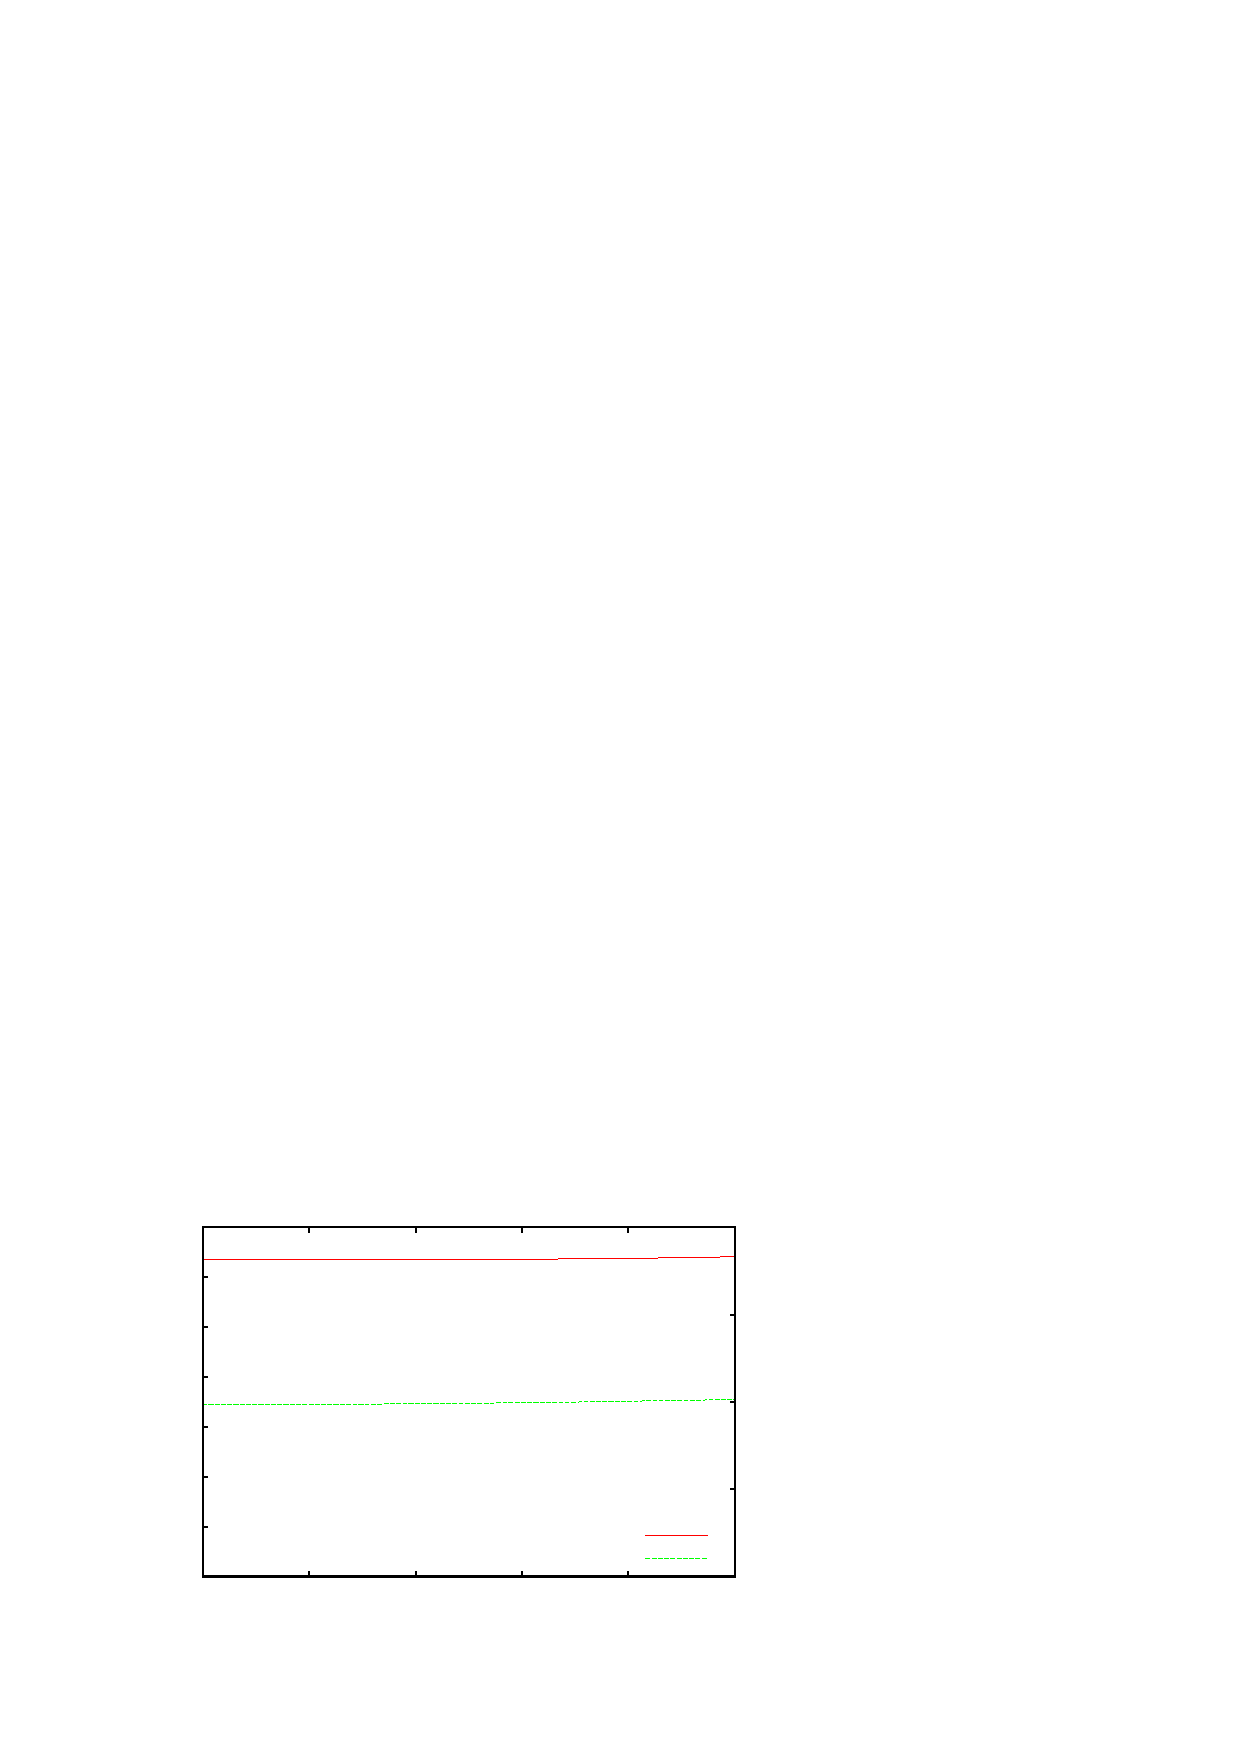
\includegraphics{./figures/e4}}%
    \gplfronttext
  \end{picture}%
\endgroup
}
\caption{Amplituden- und Phasenverhalten für $\omega=10^4 1/s$}
\end{figure}
\begin{figure}[htbp]
\centering
\scalebox{1.0}{% GNUPLOT: LaTeX picture with Postscript
\begingroup
  \makeatletter
  \providecommand\color[2][]{%
    \GenericError{(gnuplot) \space\space\space\@spaces}{%
      Package color not loaded in conjunction with
      terminal option `colourtext'%
    }{See the gnuplot documentation for explanation.%
    }{Either use 'blacktext' in gnuplot or load the package
      color.sty in LaTeX.}%
    \renewcommand\color[2][]{}%
  }%
  \providecommand\includegraphics[2][]{%
    \GenericError{(gnuplot) \space\space\space\@spaces}{%
      Package graphicx or graphics not loaded%
    }{See the gnuplot documentation for explanation.%
    }{The gnuplot epslatex terminal needs graphicx.sty or graphics.sty.}%
    \renewcommand\includegraphics[2][]{}%
  }%
  \providecommand\rotatebox[2]{#2}%
  \@ifundefined{ifGPcolor}{%
    \newif\ifGPcolor
    \GPcolortrue
  }{}%
  \@ifundefined{ifGPblacktext}{%
    \newif\ifGPblacktext
    \GPblacktextfalse
  }{}%
  % define a \g@addto@macro without @ in the name:
  \let\gplgaddtomacro\g@addto@macro
  % define empty templates for all commands taking text:
  \gdef\gplbacktext{}%
  \gdef\gplfronttext{}%
  \makeatother
  \ifGPblacktext
    % no textcolor at all
    \def\colorrgb#1{}%
    \def\colorgray#1{}%
  \else
    % gray or color?
    \ifGPcolor
      \def\colorrgb#1{\color[rgb]{#1}}%
      \def\colorgray#1{\color[gray]{#1}}%
      \expandafter\def\csname LTw\endcsname{\color{white}}%
      \expandafter\def\csname LTb\endcsname{\color{black}}%
      \expandafter\def\csname LTa\endcsname{\color{black}}%
      \expandafter\def\csname LT0\endcsname{\color[rgb]{1,0,0}}%
      \expandafter\def\csname LT1\endcsname{\color[rgb]{0,1,0}}%
      \expandafter\def\csname LT2\endcsname{\color[rgb]{0,0,1}}%
      \expandafter\def\csname LT3\endcsname{\color[rgb]{1,0,1}}%
      \expandafter\def\csname LT4\endcsname{\color[rgb]{0,1,1}}%
      \expandafter\def\csname LT5\endcsname{\color[rgb]{1,1,0}}%
      \expandafter\def\csname LT6\endcsname{\color[rgb]{0,0,0}}%
      \expandafter\def\csname LT7\endcsname{\color[rgb]{1,0.3,0}}%
      \expandafter\def\csname LT8\endcsname{\color[rgb]{0.5,0.5,0.5}}%
    \else
      % gray
      \def\colorrgb#1{\color{black}}%
      \def\colorgray#1{\color[gray]{#1}}%
      \expandafter\def\csname LTw\endcsname{\color{white}}%
      \expandafter\def\csname LTb\endcsname{\color{black}}%
      \expandafter\def\csname LTa\endcsname{\color{black}}%
      \expandafter\def\csname LT0\endcsname{\color{black}}%
      \expandafter\def\csname LT1\endcsname{\color{black}}%
      \expandafter\def\csname LT2\endcsname{\color{black}}%
      \expandafter\def\csname LT3\endcsname{\color{black}}%
      \expandafter\def\csname LT4\endcsname{\color{black}}%
      \expandafter\def\csname LT5\endcsname{\color{black}}%
      \expandafter\def\csname LT6\endcsname{\color{black}}%
      \expandafter\def\csname LT7\endcsname{\color{black}}%
      \expandafter\def\csname LT8\endcsname{\color{black}}%
    \fi
  \fi
  \setlength{\unitlength}{0.0500bp}%
  \begin{picture}(7200.00,4320.00)%
    \gplgaddtomacro\gplbacktext{%
      \csname LTb\endcsname%
      \put(814,704){\makebox(0,0)[r]{\strut{} 0}}%
      \put(814,1039){\makebox(0,0)[r]{\strut{} 5}}%
      \put(814,1374){\makebox(0,0)[r]{\strut{} 10}}%
      \put(814,1709){\makebox(0,0)[r]{\strut{} 15}}%
      \put(814,2044){\makebox(0,0)[r]{\strut{} 20}}%
      \put(814,2380){\makebox(0,0)[r]{\strut{} 25}}%
      \put(814,2715){\makebox(0,0)[r]{\strut{} 30}}%
      \put(814,3050){\makebox(0,0)[r]{\strut{} 35}}%
      \put(814,3385){\makebox(0,0)[r]{\strut{} 40}}%
      \put(814,3720){\makebox(0,0)[r]{\strut{} 45}}%
      \put(814,4055){\makebox(0,0)[r]{\strut{} 50}}%
      \put(946,484){\makebox(0,0){\strut{} 0}}%
      \put(1941,484){\makebox(0,0){\strut{} 0.02}}%
      \put(2937,484){\makebox(0,0){\strut{} 0.04}}%
      \put(3932,484){\makebox(0,0){\strut{} 0.06}}%
      \put(4928,484){\makebox(0,0){\strut{} 0.08}}%
      \put(5923,484){\makebox(0,0){\strut{} 0.10}}%
      \put(6055,704){\makebox(0,0)[l]{\strut{}$-2\pi$}}%
      \put(6055,1542){\makebox(0,0)[l]{\strut{}$-\pi$}}%
      \put(6055,2380){\makebox(0,0)[l]{\strut{} 0}}%
      \put(6055,3217){\makebox(0,0)[l]{\strut{}$\pi$}}%
      \put(6055,4055){\makebox(0,0)[l]{\strut{}$2\pi$}}%
      \put(176,2379){\rotatebox{-270}{\makebox(0,0){\strut{}Amplitude von $j$ [Fr/s/cm$^2$]}}}%
      \put(6692,2379){\rotatebox{-270}{\makebox(0,0){\strut{}Phase von $j$ [rad]}}}%
      \put(3434,154){\makebox(0,0){\strut{}Radius $\rho$ [cm]}}%
      \put(3434,3945){\makebox(0,0){\strut{}}}%
    }%
    \gplgaddtomacro\gplfronttext{%
      \csname LTb\endcsname%
      \put(4936,1097){\makebox(0,0)[r]{\strut{}\footnotesize Amplitude}}%
      \csname LTb\endcsname%
      \put(4936,877){\makebox(0,0)[r]{\strut{}\footnotesize Phase}}%
    }%
    \gplbacktext
    \put(0,0){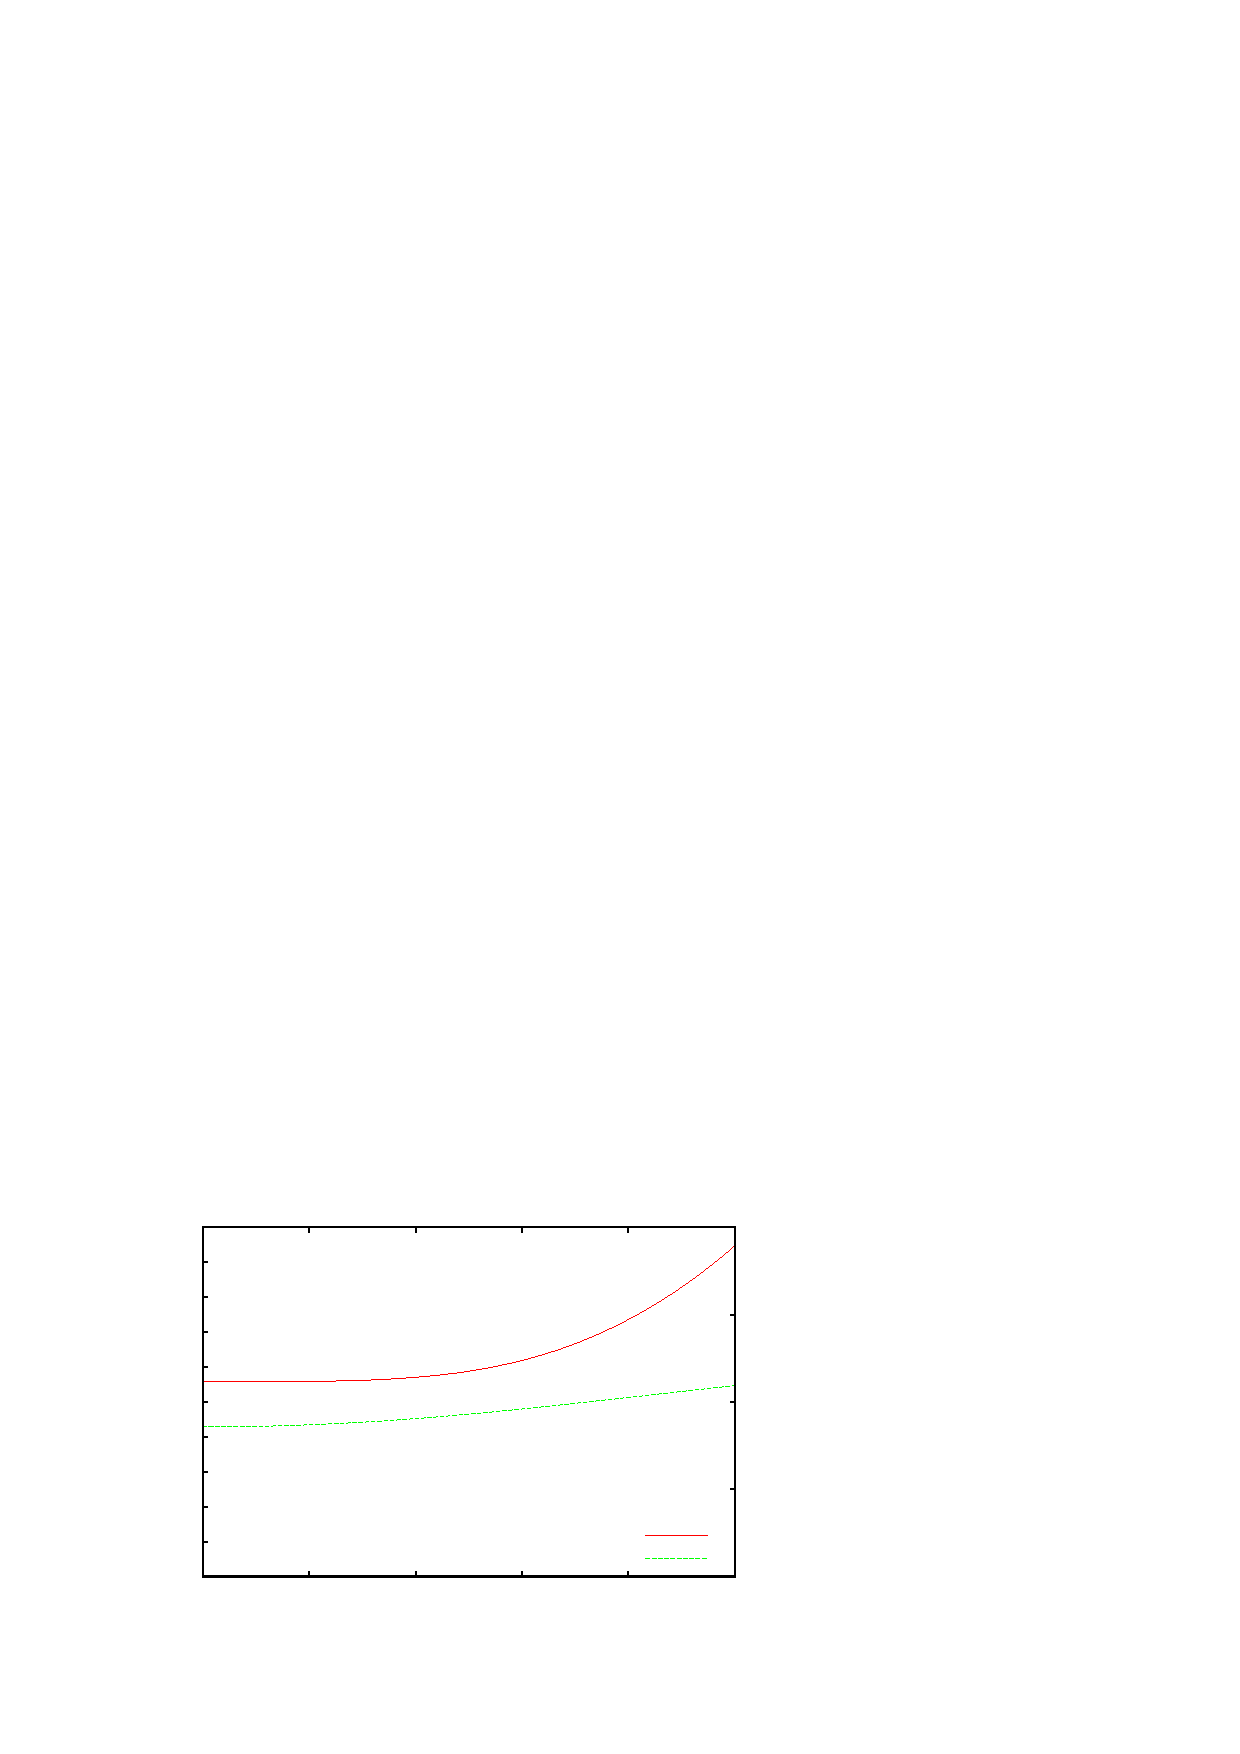
\includegraphics{./figures/e5}}%
    \gplfronttext
  \end{picture}%
\endgroup
}
\caption{Amplituden- und Phasenverhalten für $\omega=10^5 1/s$}
\end{figure}
\begin{figure}[htbp]
\centering
\scalebox{1.0}{% GNUPLOT: LaTeX picture with Postscript
\begingroup
  \makeatletter
  \providecommand\color[2][]{%
    \GenericError{(gnuplot) \space\space\space\@spaces}{%
      Package color not loaded in conjunction with
      terminal option `colourtext'%
    }{See the gnuplot documentation for explanation.%
    }{Either use 'blacktext' in gnuplot or load the package
      color.sty in LaTeX.}%
    \renewcommand\color[2][]{}%
  }%
  \providecommand\includegraphics[2][]{%
    \GenericError{(gnuplot) \space\space\space\@spaces}{%
      Package graphicx or graphics not loaded%
    }{See the gnuplot documentation for explanation.%
    }{The gnuplot epslatex terminal needs graphicx.sty or graphics.sty.}%
    \renewcommand\includegraphics[2][]{}%
  }%
  \providecommand\rotatebox[2]{#2}%
  \@ifundefined{ifGPcolor}{%
    \newif\ifGPcolor
    \GPcolortrue
  }{}%
  \@ifundefined{ifGPblacktext}{%
    \newif\ifGPblacktext
    \GPblacktextfalse
  }{}%
  % define a \g@addto@macro without @ in the name:
  \let\gplgaddtomacro\g@addto@macro
  % define empty templates for all commands taking text:
  \gdef\gplbacktext{}%
  \gdef\gplfronttext{}%
  \makeatother
  \ifGPblacktext
    % no textcolor at all
    \def\colorrgb#1{}%
    \def\colorgray#1{}%
  \else
    % gray or color?
    \ifGPcolor
      \def\colorrgb#1{\color[rgb]{#1}}%
      \def\colorgray#1{\color[gray]{#1}}%
      \expandafter\def\csname LTw\endcsname{\color{white}}%
      \expandafter\def\csname LTb\endcsname{\color{black}}%
      \expandafter\def\csname LTa\endcsname{\color{black}}%
      \expandafter\def\csname LT0\endcsname{\color[rgb]{1,0,0}}%
      \expandafter\def\csname LT1\endcsname{\color[rgb]{0,1,0}}%
      \expandafter\def\csname LT2\endcsname{\color[rgb]{0,0,1}}%
      \expandafter\def\csname LT3\endcsname{\color[rgb]{1,0,1}}%
      \expandafter\def\csname LT4\endcsname{\color[rgb]{0,1,1}}%
      \expandafter\def\csname LT5\endcsname{\color[rgb]{1,1,0}}%
      \expandafter\def\csname LT6\endcsname{\color[rgb]{0,0,0}}%
      \expandafter\def\csname LT7\endcsname{\color[rgb]{1,0.3,0}}%
      \expandafter\def\csname LT8\endcsname{\color[rgb]{0.5,0.5,0.5}}%
    \else
      % gray
      \def\colorrgb#1{\color{black}}%
      \def\colorgray#1{\color[gray]{#1}}%
      \expandafter\def\csname LTw\endcsname{\color{white}}%
      \expandafter\def\csname LTb\endcsname{\color{black}}%
      \expandafter\def\csname LTa\endcsname{\color{black}}%
      \expandafter\def\csname LT0\endcsname{\color{black}}%
      \expandafter\def\csname LT1\endcsname{\color{black}}%
      \expandafter\def\csname LT2\endcsname{\color{black}}%
      \expandafter\def\csname LT3\endcsname{\color{black}}%
      \expandafter\def\csname LT4\endcsname{\color{black}}%
      \expandafter\def\csname LT5\endcsname{\color{black}}%
      \expandafter\def\csname LT6\endcsname{\color{black}}%
      \expandafter\def\csname LT7\endcsname{\color{black}}%
      \expandafter\def\csname LT8\endcsname{\color{black}}%
    \fi
  \fi
  \setlength{\unitlength}{0.0500bp}%
  \begin{picture}(7200.00,4320.00)%
    \gplgaddtomacro\gplbacktext{%
      \csname LTb\endcsname%
      \put(946,704){\makebox(0,0)[r]{\strut{} 0}}%
      \put(946,1123){\makebox(0,0)[r]{\strut{} 20}}%
      \put(946,1542){\makebox(0,0)[r]{\strut{} 40}}%
      \put(946,1961){\makebox(0,0)[r]{\strut{} 60}}%
      \put(946,2380){\makebox(0,0)[r]{\strut{} 80}}%
      \put(946,2798){\makebox(0,0)[r]{\strut{} 100}}%
      \put(946,3217){\makebox(0,0)[r]{\strut{} 120}}%
      \put(946,3636){\makebox(0,0)[r]{\strut{} 140}}%
      \put(946,4055){\makebox(0,0)[r]{\strut{} 160}}%
      \put(1078,484){\makebox(0,0){\strut{} 0}}%
      \put(2073,484){\makebox(0,0){\strut{} 0.02}}%
      \put(3069,484){\makebox(0,0){\strut{} 0.04}}%
      \put(4064,484){\makebox(0,0){\strut{} 0.06}}%
      \put(5060,484){\makebox(0,0){\strut{} 0.08}}%
      \put(6055,484){\makebox(0,0){\strut{} 0.10}}%
      \put(6187,1542){\makebox(0,0)[l]{\strut{}$-\pi$}}%
      \put(6187,2380){\makebox(0,0)[l]{\strut{} 0}}%
      \put(6187,3217){\makebox(0,0)[l]{\strut{}$\pi$}}%
      \put(176,2379){\rotatebox{-270}{\makebox(0,0){\strut{}$|j_0(\rho)|$ [Fr/s/cm$^2$]}}}%
      \put(6692,2379){\rotatebox{-270}{\makebox(0,0){\strut{}$\phi(\rho)$ [rad]}}}%
      \put(3566,154){\makebox(0,0){\strut{}Radius $\rho$ [cm]}}%
      \put(3566,3945){\makebox(0,0){\strut{}}}%
    }%
    \gplgaddtomacro\gplfronttext{%
      \csname LTb\endcsname%
      \put(2662,3882){\makebox(0,0)[r]{\strut{}\footnotesize Amplitude}}%
      \csname LTb\endcsname%
      \put(2662,3662){\makebox(0,0)[r]{\strut{}\footnotesize Phase}}%
    }%
    \gplbacktext
    \put(0,0){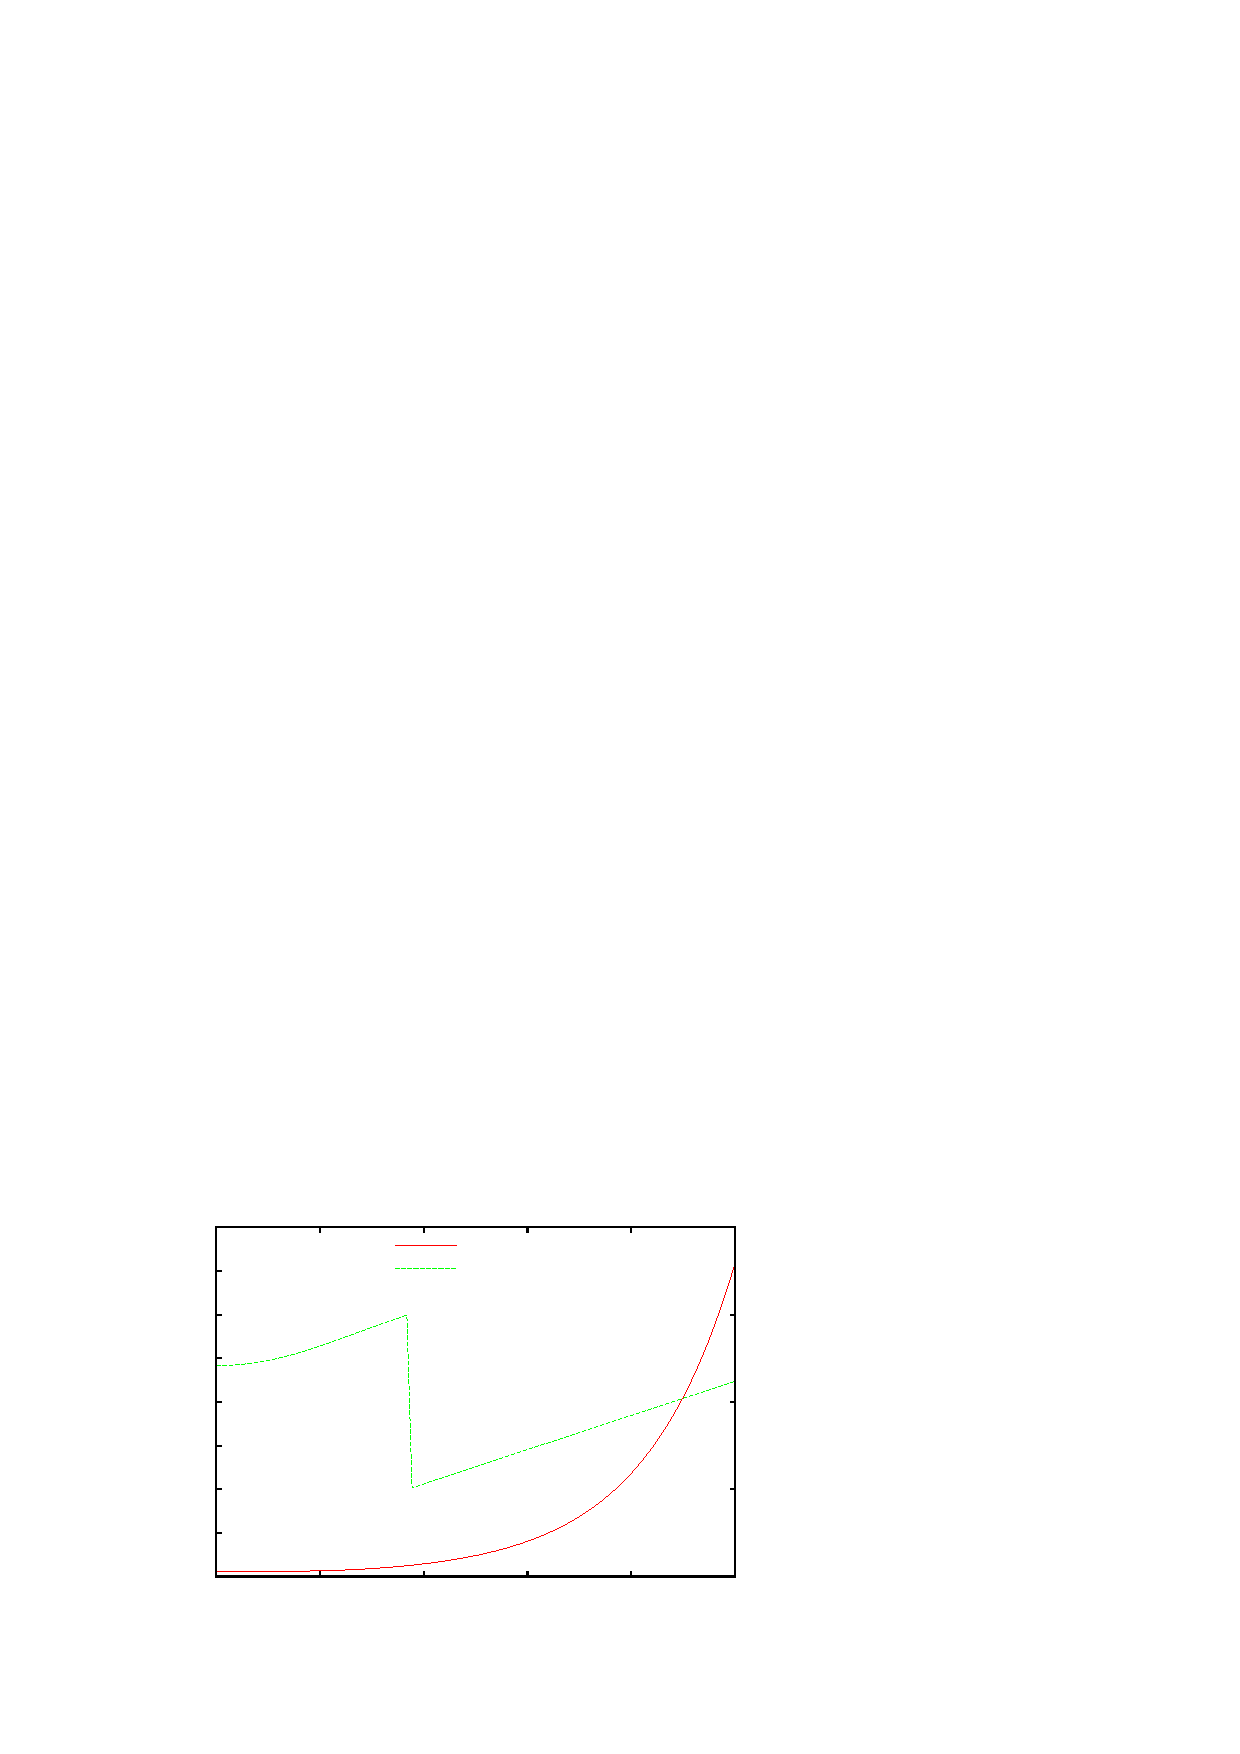
\includegraphics{./figures/e6}}%
    \gplfronttext
  \end{picture}%
\endgroup
}
\caption{Amplituden- und Phasenverhalten für $\omega=10^6 1/s$}
\end{figure}
\begin{figure}[htbp]
\centering
\scalebox{1.0}{% GNUPLOT: LaTeX picture with Postscript
\begingroup
  \makeatletter
  \providecommand\color[2][]{%
    \GenericError{(gnuplot) \space\space\space\@spaces}{%
      Package color not loaded in conjunction with
      terminal option `colourtext'%
    }{See the gnuplot documentation for explanation.%
    }{Either use 'blacktext' in gnuplot or load the package
      color.sty in LaTeX.}%
    \renewcommand\color[2][]{}%
  }%
  \providecommand\includegraphics[2][]{%
    \GenericError{(gnuplot) \space\space\space\@spaces}{%
      Package graphicx or graphics not loaded%
    }{See the gnuplot documentation for explanation.%
    }{The gnuplot epslatex terminal needs graphicx.sty or graphics.sty.}%
    \renewcommand\includegraphics[2][]{}%
  }%
  \providecommand\rotatebox[2]{#2}%
  \@ifundefined{ifGPcolor}{%
    \newif\ifGPcolor
    \GPcolortrue
  }{}%
  \@ifundefined{ifGPblacktext}{%
    \newif\ifGPblacktext
    \GPblacktextfalse
  }{}%
  % define a \g@addto@macro without @ in the name:
  \let\gplgaddtomacro\g@addto@macro
  % define empty templates for all commands taking text:
  \gdef\gplbacktext{}%
  \gdef\gplfronttext{}%
  \makeatother
  \ifGPblacktext
    % no textcolor at all
    \def\colorrgb#1{}%
    \def\colorgray#1{}%
  \else
    % gray or color?
    \ifGPcolor
      \def\colorrgb#1{\color[rgb]{#1}}%
      \def\colorgray#1{\color[gray]{#1}}%
      \expandafter\def\csname LTw\endcsname{\color{white}}%
      \expandafter\def\csname LTb\endcsname{\color{black}}%
      \expandafter\def\csname LTa\endcsname{\color{black}}%
      \expandafter\def\csname LT0\endcsname{\color[rgb]{1,0,0}}%
      \expandafter\def\csname LT1\endcsname{\color[rgb]{0,1,0}}%
      \expandafter\def\csname LT2\endcsname{\color[rgb]{0,0,1}}%
      \expandafter\def\csname LT3\endcsname{\color[rgb]{1,0,1}}%
      \expandafter\def\csname LT4\endcsname{\color[rgb]{0,1,1}}%
      \expandafter\def\csname LT5\endcsname{\color[rgb]{1,1,0}}%
      \expandafter\def\csname LT6\endcsname{\color[rgb]{0,0,0}}%
      \expandafter\def\csname LT7\endcsname{\color[rgb]{1,0.3,0}}%
      \expandafter\def\csname LT8\endcsname{\color[rgb]{0.5,0.5,0.5}}%
    \else
      % gray
      \def\colorrgb#1{\color{black}}%
      \def\colorgray#1{\color[gray]{#1}}%
      \expandafter\def\csname LTw\endcsname{\color{white}}%
      \expandafter\def\csname LTb\endcsname{\color{black}}%
      \expandafter\def\csname LTa\endcsname{\color{black}}%
      \expandafter\def\csname LT0\endcsname{\color{black}}%
      \expandafter\def\csname LT1\endcsname{\color{black}}%
      \expandafter\def\csname LT2\endcsname{\color{black}}%
      \expandafter\def\csname LT3\endcsname{\color{black}}%
      \expandafter\def\csname LT4\endcsname{\color{black}}%
      \expandafter\def\csname LT5\endcsname{\color{black}}%
      \expandafter\def\csname LT6\endcsname{\color{black}}%
      \expandafter\def\csname LT7\endcsname{\color{black}}%
      \expandafter\def\csname LT8\endcsname{\color{black}}%
    \fi
  \fi
  \setlength{\unitlength}{0.0500bp}%
  \begin{picture}(7200.00,4320.00)%
    \gplgaddtomacro\gplbacktext{%
      \csname LTb\endcsname%
      \put(946,704){\makebox(0,0)[r]{\strut{} 0}}%
      \put(946,1076){\makebox(0,0)[r]{\strut{} 50}}%
      \put(946,1449){\makebox(0,0)[r]{\strut{} 100}}%
      \put(946,1821){\makebox(0,0)[r]{\strut{} 150}}%
      \put(946,2193){\makebox(0,0)[r]{\strut{} 200}}%
      \put(946,2566){\makebox(0,0)[r]{\strut{} 250}}%
      \put(946,2938){\makebox(0,0)[r]{\strut{} 300}}%
      \put(946,3310){\makebox(0,0)[r]{\strut{} 350}}%
      \put(946,3683){\makebox(0,0)[r]{\strut{} 400}}%
      \put(946,4055){\makebox(0,0)[r]{\strut{} 450}}%
      \put(1078,484){\makebox(0,0){\strut{} 0}}%
      \put(2047,484){\makebox(0,0){\strut{} 0.02}}%
      \put(3016,484){\makebox(0,0){\strut{} 0.04}}%
      \put(3985,484){\makebox(0,0){\strut{} 0.06}}%
      \put(4954,484){\makebox(0,0){\strut{} 0.08}}%
      \put(5923,484){\makebox(0,0){\strut{} 0.10}}%
      \put(6055,704){\makebox(0,0)[l]{\strut{}$-2\pi$}}%
      \put(6055,1542){\makebox(0,0)[l]{\strut{}$-\pi$}}%
      \put(6055,2380){\makebox(0,0)[l]{\strut{} 0}}%
      \put(6055,3217){\makebox(0,0)[l]{\strut{}$\pi$}}%
      \put(6055,4055){\makebox(0,0)[l]{\strut{}$2\pi$}}%
      \put(176,2379){\rotatebox{-270}{\makebox(0,0){\strut{}Amplitude von $j$ [Fr/s/cm$^2$]}}}%
      \put(6692,2379){\rotatebox{-270}{\makebox(0,0){\strut{}Phase von $j$ [rad]}}}%
      \put(3500,154){\makebox(0,0){\strut{}Radius $\rho$ [cm]}}%
      \put(3500,3945){\makebox(0,0){\strut{}}}%
    }%
    \gplgaddtomacro\gplfronttext{%
      \csname LTb\endcsname%
      \put(4936,1097){\makebox(0,0)[r]{\strut{}\footnotesize Amplitude}}%
      \csname LTb\endcsname%
      \put(4936,877){\makebox(0,0)[r]{\strut{}\footnotesize Phase}}%
    }%
    \gplbacktext
    \put(0,0){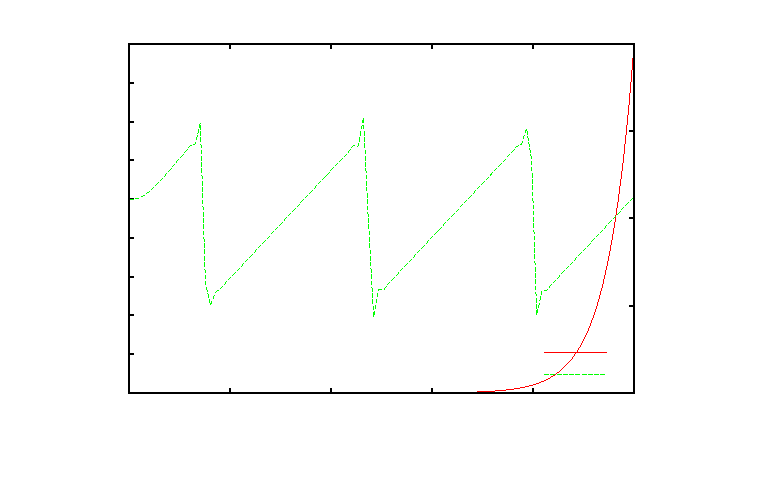
\includegraphics{./figures/e7}}%
    \gplfronttext
  \end{picture}%
\endgroup
}
\caption{Amplituden- und Phasenverhalten für $\omega=10^7 1/s$}
\end{figure}
\begin{thebibliography}{9}

\bibitem{abramowitzstegun}
Abramowitz, M. \& Stegun, I. A.
\emph{Handbook of Mathematical Functions},
Dover Books (1965)

\bibitem{healdmarion}
Heald, M. \& Marion, J.
\emph{Classical Electromagnetic Radiation},
Brooks Cole (1994)

\bibitem{kazimierczuk}
Kazimierczuk, M.
\emph{High-Frequency Magnetic Components},
Wiley (2009)

\bibitem{crchandbook}
David R. Lide (ed),
\emph{CRC Handbook of Chemistry and Physics},
84th Edition. CRC Press. Boca Raton, Florida, 2003;
Section 12, Properties of Solids; Electrical Resistivity of Pure Metals
Section 4, The Elements; Magnetic Susceptibility

\end{thebibliography}

\end{document}
